\chapter{Podstawowe Zasady UX/UI designu}

\section{Wprowadzenie do UX Designu}

 UX design, czyli projektowanie doświadczeń użytkownika, to proces tworzenia zapewniający pozytywne doświadczenia użytkownikom poprzez optymalizacje interakcji z daną stroną, systemem czy produktem. Początkowo zagadnienie to było kojarzone głównie z projektowaniem stron internetowych i aplikacji, jednak współczesne podejście znajduje zastosowanie w każdej dziedzinie. Obecnie UX design obejmuje projektowanie przeróżnych produktów, od stron internetowych po urządzenia codziennego użytku jak urządzenia AGD, samochody czy nawet meble. Aktualnie UX odnosi się nie tylko do wirtualnych interfejsów ale także do interakcji ze zwykłymi przedmiotami z którymi styczność mamy wszyscy.


\section{Podstawowe Zasady UX/UI}

Autorzy rożnych książek wyróżniają szereg fundamentalnych zasad UX designu, które pomagają w tworzeniu bardziej efektywnych, intuicyjnych i przyjemnych doświadczeń użytkowników.
Wśród kluczowych zasad projektowania UX/UI wyróżnia się:


\subsection{Ergonomia i Prostota}
Produkt powinien być projektowany tak, by był wygodny i łatwy w użyciu. Dobre projektowanie UX uwzględnia nie tylko interakcje użytkownika z urządzeniem, ale również sposób, w jaki przetwarza on informacje wyświetlane na ekranie. Produkt powinien być dostosowany do naturalnych zdolności i ograniczeń użytkownikow zapewniając im płynne i efektywne osiąganie zamierzonych celow.(Don Norman, 2013).

Zasada Prostoty oznacza elimniowanie zbędnych elementow i skomplikowanych funkcji, ktore mogą rozpraszać uwage odbiorcy lub sprawiać że produkt staje sie trudny w obsłudze. Koncentruje sie głownie na tym z czego użytkownik będzie rzeczywiscie korzystał Prostota podczas projektowania interfejsow polega na tym, ze wszystkie funkcjonalności są dostępne dla użytkownika w oczywisty i jak najprostszy sposob. Dązenie do prostoty w projekcie jest istotne ponieważ pomaga zapobiec przeciązeniu poznawczemu ktore może wystąpić gdy system jest zbyt skomplikowany. 


\subsection{Widoczność i Intuicyjność}

Dobrze zaprojektowany pod względem widoczności interfejs powinien sprawiać by użytkownik był w stanie łatwo dostrzec dostępne opcje funkcje bez konieczności szukania. Elementy powinny by umieszczone w miejscach w których naturalnie się ich spodziewają. Pozwala to na szybkie zrozumienie sposobu poruszania się w systemie. Zasada ta uwzględnia również umiejscowienie mniej istotnych elementów, takie jak ustawienia lub dodatkowe funkcje. Nie muszą one być widoczne na pierwszy rzut oka, ważne jest aby były one nadal łatwe do zlokalizowania w razie potrzeby. Don Norman

Intuicyjność oznacza, że interfejs powinien być zaprojektowany w taki sposób aby użytkownik mógł naturalnie zrozumieć jego działanie opierając się na swoich wcześniejszych doświadczeniach i oczekiwaniach. Elementy powinny być widoczne i łatwe do zlokalizowania oraz reagować zgodnie z jego przyzwyczajeniami. Sposób poruszania się po systemie powinien być dla nich oczywisty. Steve Krug

\subsection{Dostępność i Informacja zwrotna}
Zasada dostępności jest bardzo ważna, aby zapewnić by wszyscy użytkownicy, niezależnie zdolności fizycznych, sensorycznych czy poznawczych  byli w stanie korzystać z aplikacji. Treść interfejsu powinna być jasna i zrozumiała a teksty powinny być odpowiednio widoczne  z dobrym kontrastem miedzy tłem a literami. Elementy interaktywne takie jak przyciski, suwaki powinny być łatwe do znalezienia i i użyteczne. Powinien również  oferować użytkownikom dostosowania jego wyglądu , na przykład zmianę rozmiaru tekstu lub kontrastu. Designing Interfaces Jenifer Tidwell

Jest to reakcja systemu na działania, które wykonuje użytkownik pozwalając mu na kontrolowanie swoich interakcji z systemem i ich efektów w czasie rzeczywistym. Dobre projektowanie interfejsu zapewnia, że każda interakcja użytkownika, taka jak kliknięcie przycisku czy zmiana ustawienia, zostanie natychmiastowo potwierdzona odpowiednią reakcją systemu. Reakcja może przybierać różne formy, jak wizualna czy dźwiękowa.(Saffer, 2006)


\section{Róznice w projektowaniu interfejsu VR}
Chociaż większość podstawowych zasad UX designu jest uznawana jako uniwersalana to projektowanie interfejsu użytkownika w oparciu o nie wymaga od projektanta innego podejścia. Wynika to z odmienności systemu VR od innych technologii, takich jak aplikacje mobilne, aplikacje desktopowe czy strony internetowe, gdzie wszystkie interakcje z systemem odbywają się za pomocą myszki, klawiatury, ekranów dotykowych ewentualnie czytników ekranów. Tworzenie interfejsów użytkownika w środowisku wirtualnej rzeczywistości wiąże się z wieloma trudnościami, które nie występują w tradycyjnych aplikacjach. W projekcie konieczne będzie dostosowanie zasad tak, aby umożliwić użytkownikom komfortową, intuicyjną oraz płynną interakcję z produktem. Przy projektowaniu należy wziąć pod uwagę takie aspekty jak ograniczenia technologiczne i sensoryczne jak np. pole widzenia czy ograniczenia motoryczne użytkowników. 

Pierwszą fundamentalną różnicą między tradycyjnym wykorzystaniem zasad UX designu jest \textbf{Nawigacja}. W przypadku stron internetowych i aplikacji przemieszczanie się po produkcie odbywa się za pomocą klikania ikon, przewijania, ruchów myszką czy naciskania odpowiednich przycisków na klawiaturze. W wirtualnej rzeczywistości nawigowanie polega w głównej mierze na ruchach użytkownika szczególnie w przypadku bardziej zaawansowanych urządzeń takich jak  Pico 4 Ultra Enterprise, które nie wymagają dodatkowych urządzeń a korzystanie z nich odbywa się bezprzewodowo.(https://vr-expert.com/pl/samodzielne-vr/). Przemieszczanie po systemie odbywa się za pomocą śledzenia ruchow głową i ciała za pomocą kontrolerów ruchów. Często stosowane są również abstrakcyjne metody przemieszczania się, jak np. teleportacja do innego miejsca oddalonego w przestrzeni, co umożliwia eksplorowanie większych środowisk VR (Jennifer Whyte Dragana Nikolić - Virtual Reality and the Built Environment-Routledge (2018). Sam interfejs jest też inaczej umieszczony w przestrzeni. Tradycyjnie osadzone są w przestrzeni ekranu. W wirtualnej rzeczywistości interfejsy są umieszczone w przestrzeni  świata. Elementy mogą lewitować przed użytkownikiem lub częscią być częścią otoczenia. (Jonathan Linowes - Unity Virtual Reality Projects - Second Edition)
Następna równie ważna różnica to \textbf{Interakcja w przestrzeni 3D}. W tradycyjnych interfejsach  użytkownik wchodzi w interakcje z płaskimi, dwuwymiarowymi elementami na ekranie. W VR interakcje odbywają się w przestrzeni trójwymiarowej a użytkownik może dowolnie manipulować  obiektami tak jakby były on prawdziwe. Umożliwia chwytanie obracanie i przesuwanie element za pomocą rąk oraz interakcje które wymagają pełnego zaangażowania ciała użytkownika jak np. schylanie czy kucanie co wpływa pozytywnie na immersje i realizm doświadczenia.
Pozwala również na odejście od zgodności z rzeczywistością(nie wiem czy  to dobry synonim dla realizmu) i umożliwia działania niemożliwe w prawdziwym świecie jak przemieszczanie przedmiotów oddalonych w dużej odległości czy teleportacja. (Virtual, Augmented and Mixed Reality)
\textbf{Projektowanie interakcji} w wirtualnej rzeczywistości wymaga naśladowania w jaki sposob użytkownicy wchodzą w interakcje z przedmiotami i otoczeniem w prawdziwym świecie. Gesty i ruchy powinny być realistycznie odwzorowane a odpowiedz systemu natychmiastowa. Tradycyjne interakcje są bardziej pośrednie, gdy użytkownik chce wykonać jakieś działanie musi poruszyć myszką aby na ekranie kliknąć w pożądaną ikonę. W VR możliwe jest fizyczne "podniesienie" przedmiotu lub otwarcie drzwi.(Multimedia and Virtual Reality - Alistair Sutcliffe)    
W grach komputerowych czy aplikacjach rzadko zdarza się aby użytkownik odczuwał dyskomfort fizyczny, jedynym czynnikiem mogącym zakłócić poczucie komfortu jest natknięcie się na elementy wywołujące fobie, takie jak arachnofobia czy klaustrofobia. VR oferuje o wiele większą immersję niż gry na komputer i pozwala użytkownikowi na pełne zanurzenie się w rozgrywkę, ale tworzenie treści do tego środowiska wymaga zachowania większej ostrożności, aby uniknąć efektów ubocznych. Jednym z nich jest choroba symulatorowa (VR sickness).

\begin{figure}[!htb]
    \centering
    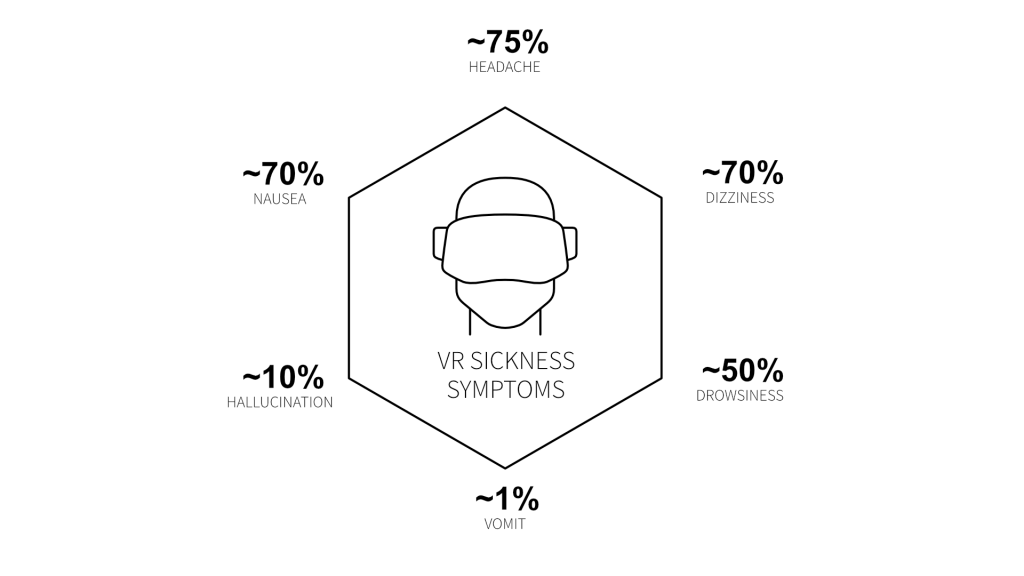
\includegraphics[width=0.8\textwidth]{images/VRSICK.png}
    \caption{Przykładowy wygląd edytora Unity}
    \label{unity_engine_example}
\end{figure}

Choroba ta jest bardzo powszechna wśród osób korzystających z wirtualnej rzeczywistości. Objawia się najczęściej mdłościami, zawrotami głowy czy ogólna dezorientacją. \textbf{}{Komfort użytkownika i jego adaptacja fizyczna} jest więc kluczowymi aspektami projektowania interfejsów użytkownika. (3D user Interfaces Theory and Practice)

Interakcje z produktami na komputery i telefony opierają się głownie na płaskich bodźcach wizualnych i dźwiękowych. Ogranicza to poziom zaangażowania odbiorcy i wpływa na mniej intensywne doświadczenia. Natomiast wirtualne środowisko może angażować nie tylko słuch i wzrok ale również dotyk poprzez kontrolery z haptyczna czy wibracje. Wirtualna rzeczywistość angażuje różne \textbf{zmysły}, aby maksymalnie zwiększyć zanurzenie użytkownika w cyfrowym świecie i zapewnić mu jak najlepsze doznania. Podane różnice dowodzą, że projektowanie interfejsu dla VR wymaga zupełnie innego podejścia niż w przypadku tradycyjnych gier i aplikacji. 


\section{Zastosowanie zasad UX do projektowania interfejsow  użytkownika w VR}

W kontekście VR projektowanie interfejsów staje się szczególnie problematyczne ze względu na konieczność osiągnięcia równowagi między imersją w wirtualnej rzeczywistości a zapewnieniem intuicyjnej interakcji oraz komfortu użytkowania, dlatego istotne jest zastosowanie sprawdzonych zasad UX dostosowanych pod to środowisko.

\subsection{Wymagania dla projektowania interfejsów VR}

Na podstawie podanych wcześniej informacji opracowano szczegołową listę wymagań które projekt musi spełniać aby interfejs był skuteczny, intuicyjny i zapewniał użytkownikom maksymalny komfort oraz immersje. 

Naturalność interakcji
Interakcje powinny naśladować  zachowania znane użytkownikom ze świata rzeczywistego. Wszelkiego rodzaju ruchy ciała, gesty i działania powinny być intuicyjne, dawać rezultaty zgodnie z oczekiwaniami użytkownika i być zgodne rzeczywistymi odczuciami ciałe. Bardzo istotny jest rownież czas reakcji i precyzja gestów, które mają ogromny wpływ na doświadczenie użytkownika. Wprowadzenie opcji teleportacji zamiast płynnego ruchu może pomóc zminimalizować różnice między tym co w VR a w prawdziwym świecie. Dobrze zaplanowane interakcje nie tylko ułatwiają korzystanie, ale również wzmacniają wrażenie obecności w świecie wirtualnym (Alistair Sutcliffe)(Jennifer Whyte, Dragana Nikolić)



Ergonomia i personalizacja

Elementy muszą być dostosowane do fizycznych ograniczen człowieka. Użytkownik powinien mieć możliwość dostosowania pod swoje preferencje i potrzeby położenia interfejsu.  Zapewni mu to większy komfort oraz znacząco wpłynie na zmniejszenie zmęczenia. Personalizacja może w tym przypadku obejmować nie tylko zmiany umiejscowienia kluczowych elementow ale rownież wykorzystywane kolorów czy rozkład elementow. Stosowanie się do zasady ergonomi zmniejsza ryzyko potencjalnych urazow wynikających z długotrwałego korzystania z VR (Virtual, Augmented and Mixed Reality Conference). 

Interfejs w wirtualnej rzeczywistości musi uwzględniać rownież rozne sposob korzystania z urządzenia takie jak siedzący, stojący lub room-scale. Można to osiągnąc poprzez umożliwienie użytkownikom manualnego dostosowania interfejsu do wzrostu i trybu w jakim urządzenie jest używane(https://vrproject.com.pl/mobilny-ux-a-vr-klucz-do-nowoczesnych-doswiadczen/).

Kolejnym ważnym aspektem o ktorym należy pamiętać jest wykorzystanie haptyki oraz dziwięku przestrzennego. 





Spójność wizualna i immersja
Interfejs powinien być spójny z wirtualnym otoczeniem i jednocześnie nie zaburzać poziomu zanurzenia. Wszystkie elementy interaktywne powinny być łatwo zauważalne, ale również nie dominować, odciągając tym samym uwagę od wykonywanych zadań.
Spójność wizualna to również wybór odpowiedniej palety kolorów oraz stylu graficznego, który skupia uwagę na odpowiednich elementach i pasującego do całego wirtualnego świata.
(Jonathan Linowes)

Wysoka wydajność i responsywność
Reakcja w witualnej rzeczywistości musi być natychmiastowa, jakiekolwiek opóźnienia mogą zaburzyć immersje i powodować u użytkownika objawy choroby symulatorowej i dyskomfort. Optymalizacja wykorzystywanych grafik i płynności jest kluczowa. Testowanie wydajności systemu i optymalizacja kodu są niezbędne aby  utrzymać jakość doświadczeń na wysokim poziomie. Warto rownmnież monitorować zuzucie zasobow sytemowych aby uniknąć przeciążenia urządzęń (Jennifer Whyte, Dragana Nikolić)

Płynność
Wysoka liczba klatek na sekunde (FPS) i minimalizacja opóźnień w śledzeniu ruchow użytkownika zmniejsza ryzyko wystąpienia objawow cybersickness. Wskazane jest utrzymanie płynności na poziomie co najmniej 90 klatek na sekunda. W przypadku bardziej zaawansowanych aplikacjach  nawet 120 fps. Oprócz wysokiej wartości FPS, należy utrzymywać niskie opóźnienie; powinno ono wynosić mniej niż 20 ms dla natychmiastowej reakcji systemu na ruchy użytkownika. Większe wartości mogą powodować opóźnienia, które dezorientują i powodują dyskomfort użytkownika.
%(https://vrpolska.eu/najwazniejsze-pojecia-vr-kadukowo/)

Optymalizacja pola widzenia (FOV) - Pole widzenia użytkownika jest istotne w zachowaniu immersji oraz redukcji efektów ubocznych korzystania z VR. Badania wykazały, że w przypadku rzeczywistości wirtualnej pole widzenia powinno wynosić od 100 do 110 stopni. Zachowanie takich wartości pozwala na zwiększenia wrażenia przebywania w wirtualnym świecie przy ograniczonym przeciążeniu sensorycznym. Zbyt szerokie pole widzenia może powodować dezorientację i zmęczenie wzroku, podczas gdy zbyt wąskie pole widzenia może ograniczać realistyczne wrażenia. Rozwiązanie musi uwzględniać niezbędne dostosowanie FOV do użytkownika i aplikacji. Szczegołowe dane na temat optymalizacji FOV znajdują sie w %(https://www.mechanik.media.pl/pliki/do_pobrania/artykuly/10/195-202.pdf)


\textbf{Czego Unikać}

Przeładowania informacjami
W VR mniej znaczy więcej, nadmierna liczba elementów w interfejsie może przytłoczyć użytkownika nadmiarem informacji i zaburzać immersję. Projektowanie do wirtualnego środowiska powinno skupiać się na minimalizmie i ograniczać do najważniejszych funkcji mniej istotne pomijając lub ukrywając. Redukcja zbędnych informacji i skupienie się na najistotniejszych funkcjonalnościach pomaga utrzymać koncentracje uzytkownika i ułatwia szybkie podejmowanie decyzji.

Nagłę zmiany perspektywy i ruchu kamery
Gwałtowne zmiany widoku mogą wywoływać dezorientacje, zawroty głowy a nawet mdłości. Poruszanie kamerą powinno odbywać się płynnie bez żadnych zakłóceń  naśladując naturalne ruchy głową użytkownika. Warto również uwzględnić stopniowe przejścia i animacje, aby zminimalizować negatywne skutki uboczne korzystania z VR. Stabilizacja i przewidywalne ruchy pomagają utrzymać komfort przez dłuższy czas. 

Brak standaryzacji interfejsów
Mimo dużej swobody w projektowaniu VR, brak spójnych i powtarzalnych zasad może frustrować użytkownikow. Należy stosować ujednolicone schematy interakcji tam gdzie to możliwe. Spojność ułatwia adaptacje do nowego środowiska, skraca to czas nauki obsługi sytemu oraz poprawia doświadzcenia użytkownika. 


%(https://www.mechanik.media.pl/pliki/do_pobrania/artykuly/10/195-202.pdf)

